\subsection{Counterfactual Reasoning}
\label{sec:cf}

Counterfactual thinking refers to imaginative thoughts about what might have been (``if only'' or ``what if'').
Counterfactual reasoning can be useful in cross-examination~\cite{Cross-Examination2021,WinArgument2006} as it allows for the examination of what could have happened if a certain event or action did not occur. This can help to identify potential biases or limitations in the information being presented and can also provide alternative perspectives on the situation being examined.

For example, if a witness is testifying about an event that they observed, a counterfactual question could be used to ask what the witness would have observed if the event had occurred in a different way. This can help to identify any potential biases in the witness's testimony and can also provide a more comprehensive understanding of the event.

Additionally, the counterfactual technique can be used in cross-examination to test the robustness of the evidence and the strength of the argument presented by the witness. It can also be used to identify the assumptions that the argument is based on and to evaluate the plausibility of the alternatives proposed. Table~\ref{tab:WhatIf} presents an example of using the counterfactual technique during cross-examination to discredit a witness's testimony. 

\begin{table}[htbp]
\caption{An Example of Counterfactual Reasoning.}
%\vspace{-.12in}
\label{tab:WhatIf}
%\resizebox{\textwidth}{!}
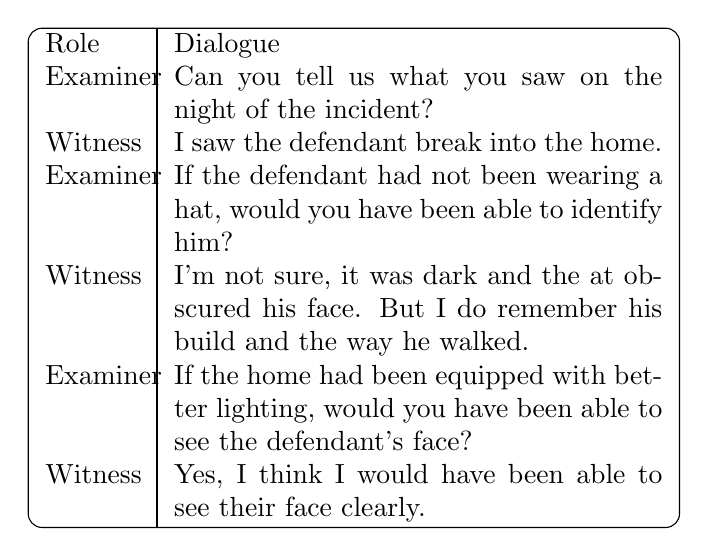
\begin{tikzpicture}
\begin{normalsize}
\node (table) [inner sep=0pt] {
\begin{tabular}{p{1.2cm}|p{6.2cm}}
\toprule
Role & Dialogue \\
\midrule
Examiner & {Can you tell us what you saw on the night of the incident?} \\
Witness & {I saw the defendant break into the home.} \\
Examiner & {If the defendant had not been wearing a hat, would you have been able to identify him?} \\
Witness & {I'm not sure, it was dark and the at obscured his face. But I do remember his build and the way he walked.} \\
Examiner & {If the home had been equipped with better lighting, would you have been able to see the defendant's face?} \\

Witness & {Yes, I think I would have been able to see their face clearly.} \\

%\bottomrule
\end{tabular}
};
\draw [rounded corners=.5em] (table.north west) rectangle (table.south east);
\end{normalsize}
\end{tikzpicture}
%\vspace{-.1in}
\end{table}

We have experimented with using the counterfactual technique to rewrite a chapter to connect the two greatest Chinese classical novels, ``Outlaws of the Marsh'' and ``Dream of the Red Chamber.'' (The example is documented
in the extended version of this paper. The citation is removed for anonymous review.)
We have also asked GPT-3 to rewrite Genesis chapter 3 by 
prompting GPT-3 that: ``What if Adam and Eve refused the serpent to eat the fruit?''
Table~\ref{tab:genesis} in Appendix A presents GPT-3's 
creativity after our ``what if'' prompt.

